% arara: pdflatex: { shell: yes }
\documentclass[twoside]{article}
\usepackage[utf8]{inputenc}
\usepackage[english]{babel}
\usepackage{amsmath, amssymb, amsthm}
\usepackage{hyperref}
\usepackage{ragged2e}
\usepackage{graphicx}
\usepackage{float}
\usepackage{fancyhdr}
\usepackage{geometry}
\usepackage{multicol}
\usepackage{url}
\usepackage{listings}
\usepackage{xcolor}
\tolerance=1000
\emergencystretch=10pt
\setlength{\headheight}{15.2pt}
\geometry{paperwidth=8.5in, paperheight=11.0in, top=1.0in, bottom=1.0in, left=1.0in, right=1.0in}

\pagestyle{fancyplain}
\fancyhead[LO]{Hackaton Coppel}
\fancyhead[CO]{}
\fancyfoot[LO]{\thepage}
\fancyfoot[CO]{Hackaton Coppel, UDLAP}
\fancyfoot[RO]{}

\begin{document}

\title{Hackaton Coppel}
\author{\small{Erick Gonzalez Parada}\\
  \small{Emiliano Ruiz Plancarte} \\
\small{Miguel Garcia Diaz de Rivera}}
\date{\today}
\maketitle

\begin{abstract}
  \raggedright
  This report analyzes a dataset provided by Coppel regarding customer service queues and times. Using data manipulation techniques, visualization, and queue theory, we propose a solution to optimize customer service attention by prioritizing elderly customers and customers who have waited beyond a threshold time. The implementation involves Python's data science stack and a custom-built priority queue system.
\end{abstract}

\begin{justify}
  \textbf{\textit{Keywords:}} Queue, DataFrame, Priority Queue, Waiting Time, Customer Service.
\end{justify}

\section{Introduction}
\subsection*{Theoretical framework}

Queueing Theory is the mathematical study of waiting lines, or queues, and has been widely used to model customer service systems \cite{queueingTheory}. It provides tools to analyze the behavior of customers and servers, helping to understand key metrics such as waiting times, service durations, and queue lengths. In practical settings, especially in customer-facing businesses like Coppel, optimizing these queues is crucial to enhance customer satisfaction and reduce operational bottlenecks.

In traditional queueing models, such as the M/M/1 model, customers are served on a first-come, first-served basis. However, real-life situations often require modifications to handle priority cases. For example, elderly customers may require special attention, or some customers may have waited excessively and deserve to be prioritized.

Our approach integrates this fundamental knowledge by constructing a \textbf{dual-priority queueing system} where:
\begin{enumerate}
    \item Elderly customers are automatically given higher priority.
    \item Non-elderly customers who have waited beyond a threshold are promoted to high priority.
\end{enumerate}

This methodology aligns with the goal of improving fairness and efficiency in service processes. By relying on Python's \textit{pandas} library for data manipulation \cite{pandas} and using the \textit{heapq} module to implement the queue structure, we can simulate and evaluate the impact of this priority mechanism.

The dataset itself was structured into a \textit{DataFrame} \cite{dataframe}, which facilitated the analysis of arrival times, service times, and customer segmentation. The priority queue implementation directly leveraged these insights to emulate more realistic queue behavior. The integration of queueing theory with actual data ensures that the solution is not only theoretically sound but also grounded in the operational reality of Coppel's service centers.


\subsection*{Goal}
The primary goal of this project is to improve customer service queue management at Coppel branches by analyzing historical service data and designing a priority queue system to optimize service order considering both elderly customers and long waiting times.

\subsection*{Materials}
\begin{itemize}
  \item \textit{Python 3} - Programming language used for analysis and implementation.
  \item \textit{Pandas} - For data manipulation and exploration \cite{pandas}.
  \item \textit{Matplotlib} - For visualization.
  \item \textit{Heapq} - For implementing the priority queue.
\end{itemize}

\subsection*{What to do}
\begin{itemize}
  \item Analyze the dataset provided by Coppel.
  \item Study customer arrival, service, and exit times.
  \item Detect potential bottlenecks.
  \item Propose a queue system prioritizing elderly people and customers with long waiting times.
\end{itemize}

\section{Methodology}
\subsection*{Dataset Overview}

\begin{figure}[H]
  \centering
  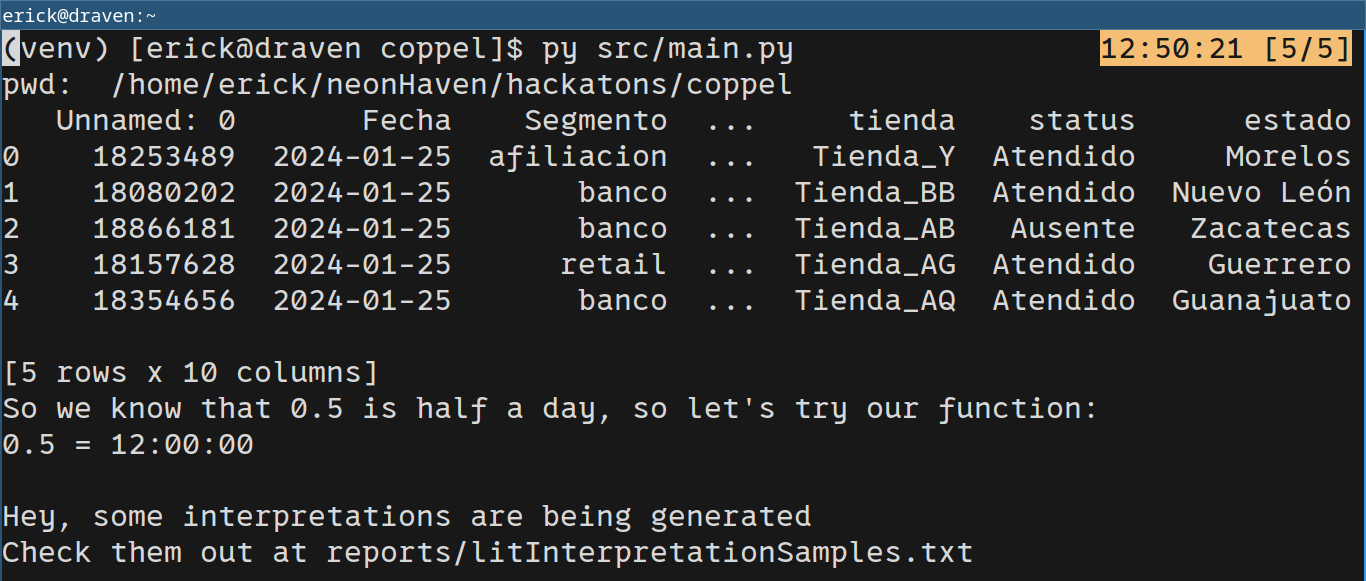
\includegraphics[width=1\textwidth]{imgs/df.png}
  \caption{dataframe head}
  \label{fig:1}
\end{figure}

The dataset provided by Coppel i.e figure \ref{fig:1}, loaded from the CSV file \texttt{v2.csv}, consists of \textbf{289,231} records with the following key columns:

\begin{itemize}
    \item \texttt{customer\_id} -- Unique customer identifier.
    \item \texttt{segment} -- Service type (\textit{banco}, \textit{retail}, \textit{afiliacion}, etc.).
    \item \texttt{isElderly} -- Indicates if the customer is elderly (boolean).
    \item \texttt{arrivalTime}, \texttt{serviceStartTime}, \texttt{serviceEndTime} -- Time fields expressed as fractions of a day.
\end{itemize}

Exploratory analysis shows:
\begin{itemize}
    \item The majority of services belong to the \textit{banco} and \textit{retail} segments.
    \item Around 12\% of customers are elderly.
    \item Average waiting time ranges between 7 to 10 minutes depending on the segment.
    \item Service durations follow a slightly skewed distribution with most services taking between 5 and 15 minutes.
\end{itemize}

This information is crucial to justify the design of our dual-priority system, where elderly customers and long-waiting customers are handled more efficiently.


We used Python's Pandas library to load and preprocess the dataset. Missing values were identified, and new features such as \textit{waitTime}, \textit{serviceTime}, and \textit{totalTime} were computed. Exploratory Data Analysis (EDA) was performed to understand distributions of segments, service statuses, and store performance. Finally, we implemented a custom priority queue simulating a real queue at a service branch.

\section{Proposed Solution}
The proposed solution is based on queueing theory \cite{queueingTheory}. The system prioritizes:
\begin{enumerate}
    \item Elderly customers (marked with an \texttt{isElderly} attribute).
    \item Customers who have waited longer than a specified threshold.
\end{enumerate}
This dual-priority system helps ensure fair and efficient service. We implemented it using Python's \texttt{heapq} module, which allows dynamic updating of customer priorities based on waiting time.

\subsection*{Interpretation}
Each row in the dataset represents a customer. We converted numerical time formats into human-readable timestamps. For instance, if a customer arrives at \texttt{0.5} (fraction of a day), it corresponds to 12:00 PM.

\begin{figure}[H]
  \centering
  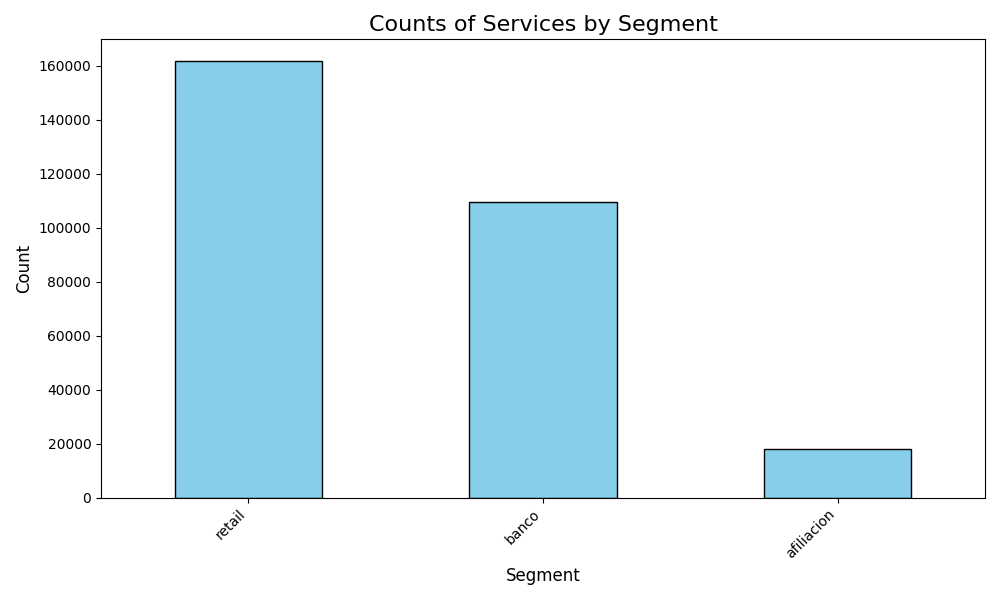
\includegraphics[width=1\textwidth]{imgs/segmentCountsPlot.png}
  \caption{Count of Services by Segment}
  \label{fig:2}
\end{figure}

The data shows that:
\begin{itemize}
    \item The dataset consists of \textbf{289,231} records.
    \item Average customer wait time is roughly 7-10 minutes depending on the segment.
    \item According to figure \ref{fig:2} the most common segments are \textit{banco}, \textit{retail}, and \textit{afiliacion}.
\end{itemize}


\subsection*{Priority Queue Simulation}
The queue dynamically adjusts as customers are added:
\begin{itemize}
    \item If a customer is elderly, they automatically get high priority.
    \item If a non-elderly customer waits beyond the defined threshold (e.g., 10 minutes), they are escalated to high priority.
    \item The queue maintains a balanced service between elderly customers and those who waited too long.
\end{itemize}

\begin{figure}[H]
  \centering
  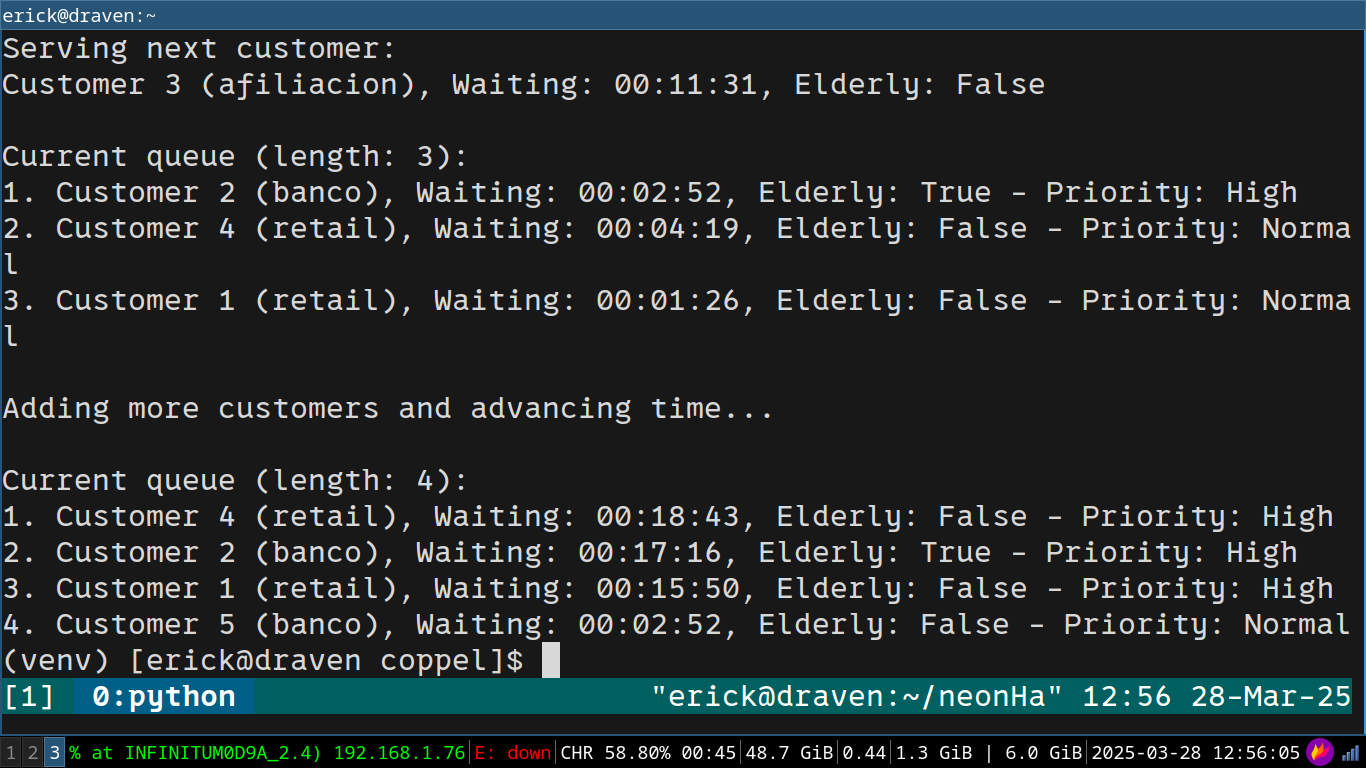
\includegraphics[width=1\textwidth]{imgs/outpOfSol.png}
  \caption{Fragment of output of solution.py}
  \label{fig:3}
\end{figure}

This solution reduces waiting time unfairness and can be adapted in real-time to suit Coppel's service flow.

\section{Access to Source Code}
The source code for this project is publicly available on GitHub at \url{https://github.com/HugeErick/CoppelHackaton}. The repository includes:
\begin{itemize}
    \item Data processing scripts.
    \item Priority queue implementation.
    \item Visualization tools.
    \item Sample interpretations.
\end{itemize}
Follow the instructions in the README to reproduce the results.

\section{Conclusions}
This project successfully demonstrates how data analysis combined with queueing theory can improve customer service. By prioritizing elderly customers and customers who have waited excessively, service becomes fairer and more efficient. The system is adaptable and could be implemented in Coppel's real operations after testing.

\begin{thebibliography}{9}
  \bibitem{pandas}
  Pandas. (n.d.). PyPI. Retrieved March 28, 2025, from \url{https://pypi.org/project/pandas/}
  
  \bibitem{dataframe}
  Pandas DataFrame. (2024, June 13). GeeksforGeeks. Retrieved from \url{https://www.geeksforgeeks.org/python-pandas-dataframe/}
  
  \bibitem{queueingTheory}
  Queuing theory. (2024, May 27). GeeksforGeeks. Retrieved from \url{https://www.geeksforgeeks.org/queuing-theory/} 
\end{thebibliography}

\end{document}

